\documentclass{article} % For LaTeX2e
% \usepackage{hyperref}
\usepackage{url}
\usepackage{amssymb,amsmath}
\pdfoutput=1
\usepackage[pdftex]{graphicx}
\usepackage{algorithm}
\usepackage{algpseudocode}
\usepackage[margin=1in]{geometry}

\title{Neuron's Eye View: Inferring Features of Complex Stimuli from Neural Responses}

\author{
John M.~Pearson\\
Duke Institute for Brain Sciences \\
Duke University\\
Durham, NC 27708 \\
\texttt{john.pearson@duke.edu} \\
\\
Jeffrey M.~Beck \\
Department of Neurobiology \\
Duke University Medical Center \\
Durham, NC 27708 \\
\texttt{jeff.beck@duke.edu} \\
}

\begin{document}

\maketitle

\begin{abstract}
Experiments that study neural encoding of stimuli at the level of individual neurons typically choose a small set of features present in the world --- contrast and luminance for vision, pitch and intensity for sound --- and assemble a stimulus set that systematically (and preferably exhaustively) varies along these dimensions. Neuronal responses in the form of firing rates are then examined for modulation with respect to these features via some form of regression. This approach requires that experimenters know (or guess) in advance the relevant features coded by a given population of neurons. Unfortunately, for domains as complex as social interaction or natural movement, the relevant feature space is poorly understood, and an arbitrary \emph{a priori} choice of feature sets may give rise to confirmation bias. Here, we present a Bayesian model for exploratory data analysis that is capable of automatically identifying the features present in unstructured stimuli based solely on neuronal responses. Our approach is unique within the class of latent state space models of neural activity in that it assumes that firing rates of neurons are sensitive to multiple discrete time-varying features tied to the \emph{stimulus}, each of which has Markov (or semi-Markov) dynamics. That is, we are modeling stimulus dynamics as driven by neural activity, rather than intrinsic neural dynamics.  We derive a fast variational Bayesian inference algorithm and show that it correctly recovers hidden features in synthetic data, as well as ground-truth stimulus features in a prototypical neural dataset. To demonstrate the utility of the algorithm, we also apply it to an exploratory analysis of prefrontal cortex recordings performed while monkeys watched naturalistic videos of primate social activity.
\end{abstract}

\section{Introduction}
The question of how the brain encodes information from the natural world forms one of the primary areas of study within neuroscience. For many sensory systems, particularly vision and audition, the discovery that single neurons modulate their firing of action potentials in response to particular stimulus features has proven foundational for theories of sensory function. Indeed, neuronal responses to contrast, edges, and motion direction appear to form fundamental primitives on which higher-level visual abstractions are built. Nevertheless, many of these higher-level abstractions, increasingly of interested to modern neuroscience, do not exist in a stimulus space with obvious axes. As a result, experimentalists must choose \emph{a priori} features of interest in constructing their stimulus sets, with the result that cells may appear weakly tuned due to misalignment of stimulus and neural axes.

For example, in vision, methods like reverse correlation have proven successful in elucidating response properties of some cell types, but such techniques rely on a well-behaved stimulus space and a highly constrained encoding model in order to achieve sufficient statistical power to perform inference \cite{steveninck1988realtime,ringach2004reverse,ringach2002receptive}. However, natural stimuli are known to violate both criteria, generating patterns of neural activity that differ markedly from those observed in controlled experiments with limited stimulus complexity \cite{ringach2002receptive,sharpee2004analyzing,Vinje2000-dx}. Information-based approaches have gone some way in addressing this challenge \cite{sharpee2004analyzing}, but this approach assumes a metric structure on stimuli in order to perform optimization, and was recently shown to be strongly related to standard Poisson regression models\cite{Williamson2013-rg}.

More recently, Gallant and collaborators have tackled this problem in the context of fMRI, demonstrating that information present in the blood oxygen level-dependent (BOLD) signal is sufficient to classify and map the representation of natural movie stimuli across the brain \cite{Vu2011-da,Huth2012-cj,Stansbury2013-nm}. These studies have used a number of modeling frameworks, from latent dirichlet allocation for categorizing scene contents \cite{Stansbury2013-nm} to regularized linear regression \cite{Huth2012-cj} to sparse nonparametric models \cite{Vu2011-da} in characterizing brain encoding of stimuli, but in each case, models were built on pre-labeled training data. Clearly, a method that could infer stimulus structure directly from neural data themselves could extend such work to include less easily characterized stimulus sets like those depicting social interactions.

Another recent line of work, this one focused on latent Poisson processes, has addressed the task of modeling the low dimensional dynamics of neural populations\cite{Pillow2008-em,Vogelstein2009-ax,Park2014-el,Buesing2014-ta}. Using generalized linear models and latent linear dynamical systems as building blocks, these models have proven able to infer (functional) connectivity \cite{Pillow2008-em}, estimate spike times from a calcium images\cite{Vogelstein2009-ax}, and identify subgroups of neurons that share response dynamics\cite{Buesing2014-ta}. Inference in thsese models is generally performed via expectation maximization, though \cite{Ulrich2014-zc} and \cite{Putzky2014-up} also used a variational Bayesian approach. Our work is distinct from those models, however, in that both were concerned with modeling and discriminating \emph{internal} states based on neural responses, while this work focuses on detecting features in \emph{external} stimuli. 

Our model sits at the intersection of these regression and latent variable approaches. We utilize a Poisson observation model that shares many of the same features as the commonly used generalized linear models for Poisson regression. We also assume that the latent features modulating neural activity are time-varying and Markov. However, we make 3 additional unique assumptions: First, we assume that the activity of each neuron is modulated by a combination of multiple independent latent features governed by semi-Markov dynamics. This allows for latents to evolve over multiple timescales with non-trivial duration distributions, much like the hand-labeled features in social interaction data sets. Second, we assume that these latents are tied to stimulus presentation. That is, when identical stimuli are presented, the same latents are also present. This allows us to model the daynamics of latent features of the \emph{stimulus} that drive neural activity, rather than intrinsic neural dynamics. Finally, we enforce a sparse hierarchical prior on modulation strength that effectively limits the number of latent features to which the population of neurons is selective. This allows for a parsimonious explanation of the firing rates of single units in terms of a small set of stimulus features. Finally, we perform full variational Bayesian inference on all model parameters and take advantage of conditional conjugacy to generate coordinate ascent update rules, nearly all of which are explicit. Combined with forward-backward inference for latent states, our algorithm is exceptionally fast, automatically implements Occam's razor, and facilitates proper model comparisons using the variational lower bound.

\section{Model}
\label{model_sec}
\begin{figure}[ht]
    \center
    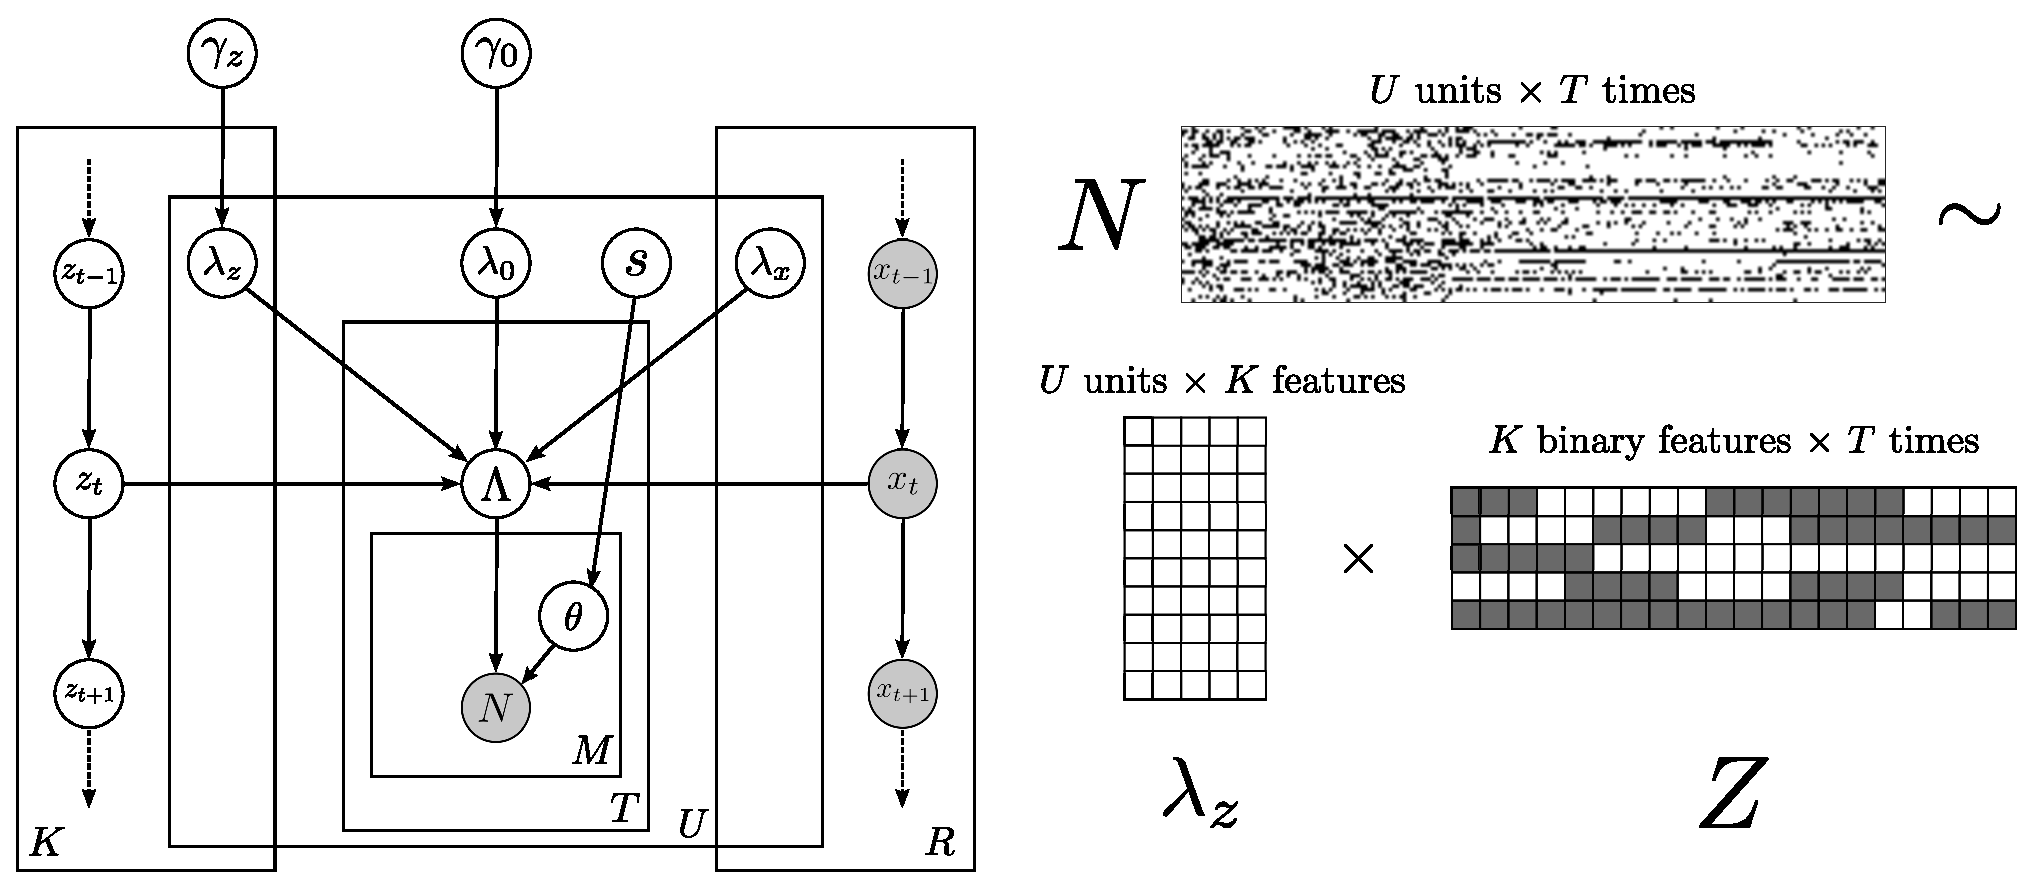
\includegraphics[width=1\linewidth]{model}
    \caption{\textbf{Generative model for spike counts.} Spike counts $N$ are observed for each of $U$ units over stimulus time $T$ for multiple presentations $M$. Counts are assumed Poisson-distributed, with firing rates $\Lambda$ that depend on each unit's responses ($\lambda$) to both latent discrete states $z_t$ and observed covariates $x_t$ that change in time, as well as a baseline firing rate $\lambda_0$. $\gamma$ nodes represent hyperparameters for the firing rate effects. $\theta$ is a multiplicative overdispersion term specific to each observation, distributed according to hyperparameters $s$.}
\end{figure}
\subsection{Observation model}
Consider a population of $U$ spiking neurons exposed to a series of stimuli indexed by a (unique) time index $t\in \lbrace 1\ldots T\rbrace$. Each neuron is exposed to each stimulus $M_{tu}$ times, where we do not assume either that each neuron observes each stimulus time or that consecutive times are observed by the same sets of neurons. That is $M_{tu}$ may have many 0s. For each observation $m$ (a unique unit, time pair), we then observe a spike count, $N_m$. We model these spike counts as arising from a Poisson process with time-dependent rate $\Lambda_{tu}$ and observation-specific multiplicative overdispersion $\theta_m$:
\begin{align}
    \label{obs_model}
    N_{m} &\sim \text{Pois}(\Lambda_{t(m), u(m)} \theta_m) &
    \theta_m &\sim \text{Ga}(s_{u(m)}, s_{u(m)})
\end{align}
Note that both the unit and time are functions of the observation index, $m$, and that the distribution of the overdispersion for each observation is specific to the unit observed. 

\subsection{Firing rate model}
At each stimulus time $t$, we assume the existence of $K$ binary latent states $z_{tk}$ and $R$ observed covariates $x_{tr}$. We further assume that each unit's firing rate response at each time can be modeled as arising from the product of three effects: (1) a baseline firing rate specific to each unit, (2) a product of responses to each latent state, and (3) a product of responses to each observed covariate:
\begin{equation}
    \label{fr_model}
    \Lambda_{tu} = \lambda_{0u} \prod_{k = 1}^K \lambda_{zuk}^{z_{tk}}  
    \prod_{r = 1}^R \lambda_{xur}^{x_{tr}}   
\end{equation} 
Note that this is conceptually similar to the generalized linear model for firing rates (in which we model $\log \Lambda$) with the identification $\beta = \log \lambda$. However, by modeling the firing rate as a product and placing Gamma priors on the individual effects, we will be able to take advantage of closed-form variational updates resulting from conjugacy that avoid explicit optimization (see below). 

In addition, to enforce parsimony in the inferred features, we put sparse hierarchical priors with hyperparameters $\gamma = (c, d)$ on the $\lambda_z$ terms:
\begin{align}
    \label{hierarchy}
    \lambda_{zuk} &\sim \text{Ga}(c_{zk}, c_{zk} d_{zk}) & c_{zk} &\sim \text{Ga}(a_{ck}, b_{ck})
    & d_{zk} &\sim \text{Ga}(a_{dk}, b_{dk})
\end{align}
That is, $\mathbb{E}[\lambda_u] = d^{-1}$ and $\text{var}[\lambda_u] = (cd^2)^{-1}$, so for $c$ large and $d\sim \mathcal{O}(1)$, the prior for firing rate response to each latent feature will be strongly concentrated around gain 1 (no effect). And once again, this choice of priors will lead to closed-form updates in our variational approximation. Finally, for the baseline terms, $\lambda_{0u}$, we use a non-sparse version of the same model, while for the specified covariate responses, $\lambda_{xu}$, we model the unit effects non-hierarchially, using independent Gamma priors for each unit.

\subsection{Latent state model}
We model each of the latent states $z_{tk}$ as an independent Markov process for each feature $k$. That is, each $k$ indexes an independent Markov chain with initial state probability $\pi_k\sim \text{Dir}(\alpha_\pi)$ and transition matrix $A_k\sim \text{Dir}(\alpha_A)$. For the semi-Markov case, we assume that the dwell times in each state are distributed independently for each chain according to an integer-valued, truncated lognormal distribution with support on the integers $1\dots D$:
\begin{align}
    \label{semi-markov}
    p_k(d|z = j) &= \text{Log-Normal}(d|m_{jk}, s^2_{jk}) / W_{jk}  &
    W_{jk} &= \sum_{d = 1}^D \text{Log-Normal}(d|m_{jk}, s^2_{jk}) 
\end{align}
Note that we have allowed the dwell time distribution to depend on both the feature $k$ and the state of the Markov chain $j$. In addition, we put indpendent Normal-Gamma priors on the mean $(m_{kj})$ and precision $(\tau_{kj} \equiv s_{kj}^{-2})$ parameters of the distribution: $(m, \tau) \sim \text{NG}(\mu, \lambda, \alpha, \beta)$.

\section{Inference}

We perform variational inference for the posteriors over the model parameters $\Theta = (\lambda_0, \lambda_z, \lambda_x, A, \pi, c_0, d_0, c_z, d_z, s)$ and latents $Z=(z_{kt},\theta_m)$. In addition, for the semi-Markov case, we include $(m, \tau)$, the parameters for the state dwell time distribution. That is, we wish to approximate the joint posterior density, 
\begin{equation}
    p(\Theta,Z|N) \propto p(N, Z |\lambda, A, \pi, \theta, \gamma) 
    p(\lambda|\gamma) p(\gamma)
    p(A)p(\pi)p(\theta|s)p(s)
\end{equation}

by a variational posterior $q_\Theta(\Theta)q_Z(Z)$ that factorizes over parameters and latents but is nonetheless close to $p$ as measured by the Kullback-Leibler divergence \cite{Wainwright2008-ii}. Equivalently, we wish to maximize the variational objective

\begin{equation}
    \mathcal{L} \equiv \mathbb{E}_q \left[\log \frac{p(\Theta,Z|N)}{q_\Theta(\Theta)q_Z(Z,\theta)} \right] = \mathbb{E}_q \left[\log p(\Theta,Z|N) \right] + \mathcal{H}[q_\Theta(\Theta)] + \mathcal{H}[q_Z(Z)]
\end{equation}

with $\mathcal{H}$ the entropy. Following the factorial HMM work of \cite{ghahramani1997factorial}, we also assume that the posterior factorizes over each latent time series $z_{\bullet k}$ and the overdispersion factor $\theta_m$, as well as the rate parameters $\lambda_{\bullet u \bullet}$ associated with each Markov process.  This factorization results in a variational posterior of the form:

\begin{multline}
    q(\Theta,Z) = q(c_0)q(d_0)\prod_m q(\theta_m) \prod_u q(s_u) q(\lambda_{0u}) \prod_r q(\lambda_{xur}) \times \\ 
    \prod_k q(c_k) q(d_k) 
    q(\lambda_{zuk}) q(c_{zk}) q(d_{zk}) q(z_k) q(\pi_k) q(A_k)
\end{multline}
With this ansatz, the variational objective decomposes in a natural way, and choices are available for many of the $q$s that lead to closed-form updates.

\subsection{Variational posterior}
From \ref{obs_model} and \ref{fr_model} above, we can write the probability of the observed data $N$ as
\begin{multline}
    \label{log_evidence}
    \log p(N, z|x, \Theta) = \sum_{mkr} \left[ 
        N_m \left( \log \theta_m +
            \log \lambda_{0u(m)} +
            z_{t(m) k} \log \lambda_{zu(m) k} + 
            x_{t(m) r} \log \lambda_{xu(m) r}
            \right)
    \right] \\
    - \sum_m \theta_m \Lambda_{t(m) u(m)} + 
    \sum_{mk} \log (A_k)_{z_{t(m)+1, k}, z_{t(m), k}} + 
    \sum_k \log (\pi_k)_{z_{0k}} + \text{constant,}
\end{multline}
where again, $m$ indexes observations of (time, unit) pairs and the last two nontrivial terms represent the probability of the Markov sequence given by $z_{tk}$. Given that \ref{log_evidence} is of an exponential family form for $\theta$ and $\lambda$ conditioned on all other variables, free-form variational arguments \cite{Wainwright2008-ii} suggest variational posteriors:
\begin{align}
    \lambda_{0u} &\sim \text{Ga}(\alpha_{0u}, \beta_{0u}) &
    \lambda_{zuk} &\sim \text{Ga}(\alpha_{zuk}, \beta_{zuk}) &
    \lambda_{xur} &\sim \text{Ga}(\alpha_{xur}, \beta_{xur})
\end{align}
For the first of these two, updates in terms of expected sufficient statistics involving expectations of $\gamma = (c, d)$ are straightforward (see Supplement). However, this relies on the fact that $z_t \in \lbrace0, 1\rbrace$. The observed covariates $x_t$ follow no such restriction, which results in a transcendental equation for the $\beta_x$ updates which we solve using an explicit BFGS optimization on each iteration. Moreover, we place non-hierarchical Gamma priors on these effects: $\lambda_{xur} \sim \text{Ga}(a_{xur}, b_{xur})$.

As stated above, we place hierarchical priors on $\lambda_0$, $\lambda_z$, and $\theta$ of the form Eq. \ref{hierarchy} that tie the hyperparameters for rate parameters $\lambda$ and overdispersion effects $\theta$ across units.  This involves multiple terms in the expected log evidence of the form
\begin{equation}
    \mathbb{E}_q \left[\sum_u \log p(\lambda_u|c, d)\right] = \sum_u \mathbb{E}_q \left[ 
    (c - 1) \log \lambda_u - cd\lambda_u + c \log cd - \log \Gamma(c) 
    \right] 
\end{equation}
In order to calculate the expectation, we make use of the inequality %\cite{abramowitz1964handbook}
\begin{equation}
    \sqrt{2\pi} \le \frac{z!}{z^{z+\frac{1}{2}} e^{-z}} \le e
\end{equation}
to lower bound the negative gamma function and approximate the above as
\begin{equation}
    \log p(\lambda) \ge \sum_u \left[ 
    (c - 1) (\log \lambda_u + 1) - cd\lambda_u + c \log d + \frac{1}{2}\log c\right]
\end{equation}
Clearly, the conditional probabilities for $c$ and $d$ are gamma in form, so that if we use priors $c \sim \text{Ga}(a_c, b_c)$ and $d\sim \text{Ga}(a_d, b_d)$ the posteriors have the form
\begin{align}
    c &\sim \text{Ga}\left(a_c + \frac{U}{2}, 
    b_c + \sum_u\mathbb{E}_q 
        \left[d \lambda_u - \log \lambda_u - \log d - 1\right]\right) \\
    d &\sim \text{Ga}\left(
        a_d + U\mathbb{E}_q[c], b_d + \sum_u \mathbb{E}_q [c \lambda_u]
    \right)
\end{align}
This basic form, with appropriate indices added, gives the update rules for the hyperparameter posteriors for $\lambda_0$ and $\lambda_z$. For $\theta$, we simply set $c = s_u$ and $d = 1$.

\subsection{Latent state inference}
For Hidden Markov Models, given the observation model \ref{log_evidence}, inference for $z$, $A$, and $\pi$ for each latent feature can be performed efficiently via conjugate updates and the well-known forward-backward algorithm \cite{beal2003variational}. For the case of semi-Markov dynamics, we additionally need to perform inference on the parameters $(m, \tau)$ of the dwell time distributions for each state. In the case of continuous dwell times, our model \ref{semi-markov} would have $W = 1$ and be conjugate to the Normal-Gamma prior on $(m, \tau)$, but the restriction to discrete dwell times requires us to again lower bound the variational objective:
\begin{equation}
    \mathbb{E}_q\left[-\log W_{jk} \right] = 
    \mathbb{E}_q\left[- \log \left( \sum_{d=1}^D p(d|j)\right) \right]
    \ge -\log \sum_{d = 1}^D \mathbb{E}_q\left[p(d|j)\right]
\end{equation}
This correction for trunction must then be added to $\mathbb{E}_q[p(z|\Theta)]$. For inference in the semi-Markov case, we use an extension of the forward-backward algorithm\cite{Yu2006-bb}, at the expense of computational complexity $\mathcal{O}(SDT)$ $(S = 2)$ per latent state, to calculate $q(z_k)$ (see Supplement). For the $4SK$ hyperparameters of the Normal-Gamma distribution, we perform an explicit BFGS optimization on the $4S$ parameters of each chain on each iteration.

\section{Experiments}
\subsection{Synthetic data}
We generated synthetic data from the model in Section \ref{model_sec} for $U=100$ neurons for $T=10,000$ time bins of $dt=0.0333s$ ($\approx 6$min). Assumed firing rates and effect sizes were realistic for cortical neurons, with mean baseline rates of 10 spikes/s and firing rate effects given by a $\text{Ga}(1, 1)$ distribution for $K_{\text{data}}=3$ latent features. In addition, we included $R=3$ known covariates generated according to Markov dynamics. For this experiment, we assumed that each unit was presented once with the stimulus time series, so that $M = 1$. That is, we tested a case in which inference was driven primarily by variabiliy in population responses across stimuli rather than pooling of data across repetitions of the same stimulus. Moreover, to test the model's ability to parsimoniously infer features, we set $K=5$. That is, we asked the model to recover more features than were present in the data. Finally, we placed hierarchical priors on unit baseline firing rates and sparse hierarchical priors on firing rate effects of latent states. We used 5 random restarts and iterated over parameter updates until the fractional change in $\mathcal{L}$ dropped below $10^{-4}$.

\begin{figure}[ht]
    \center
    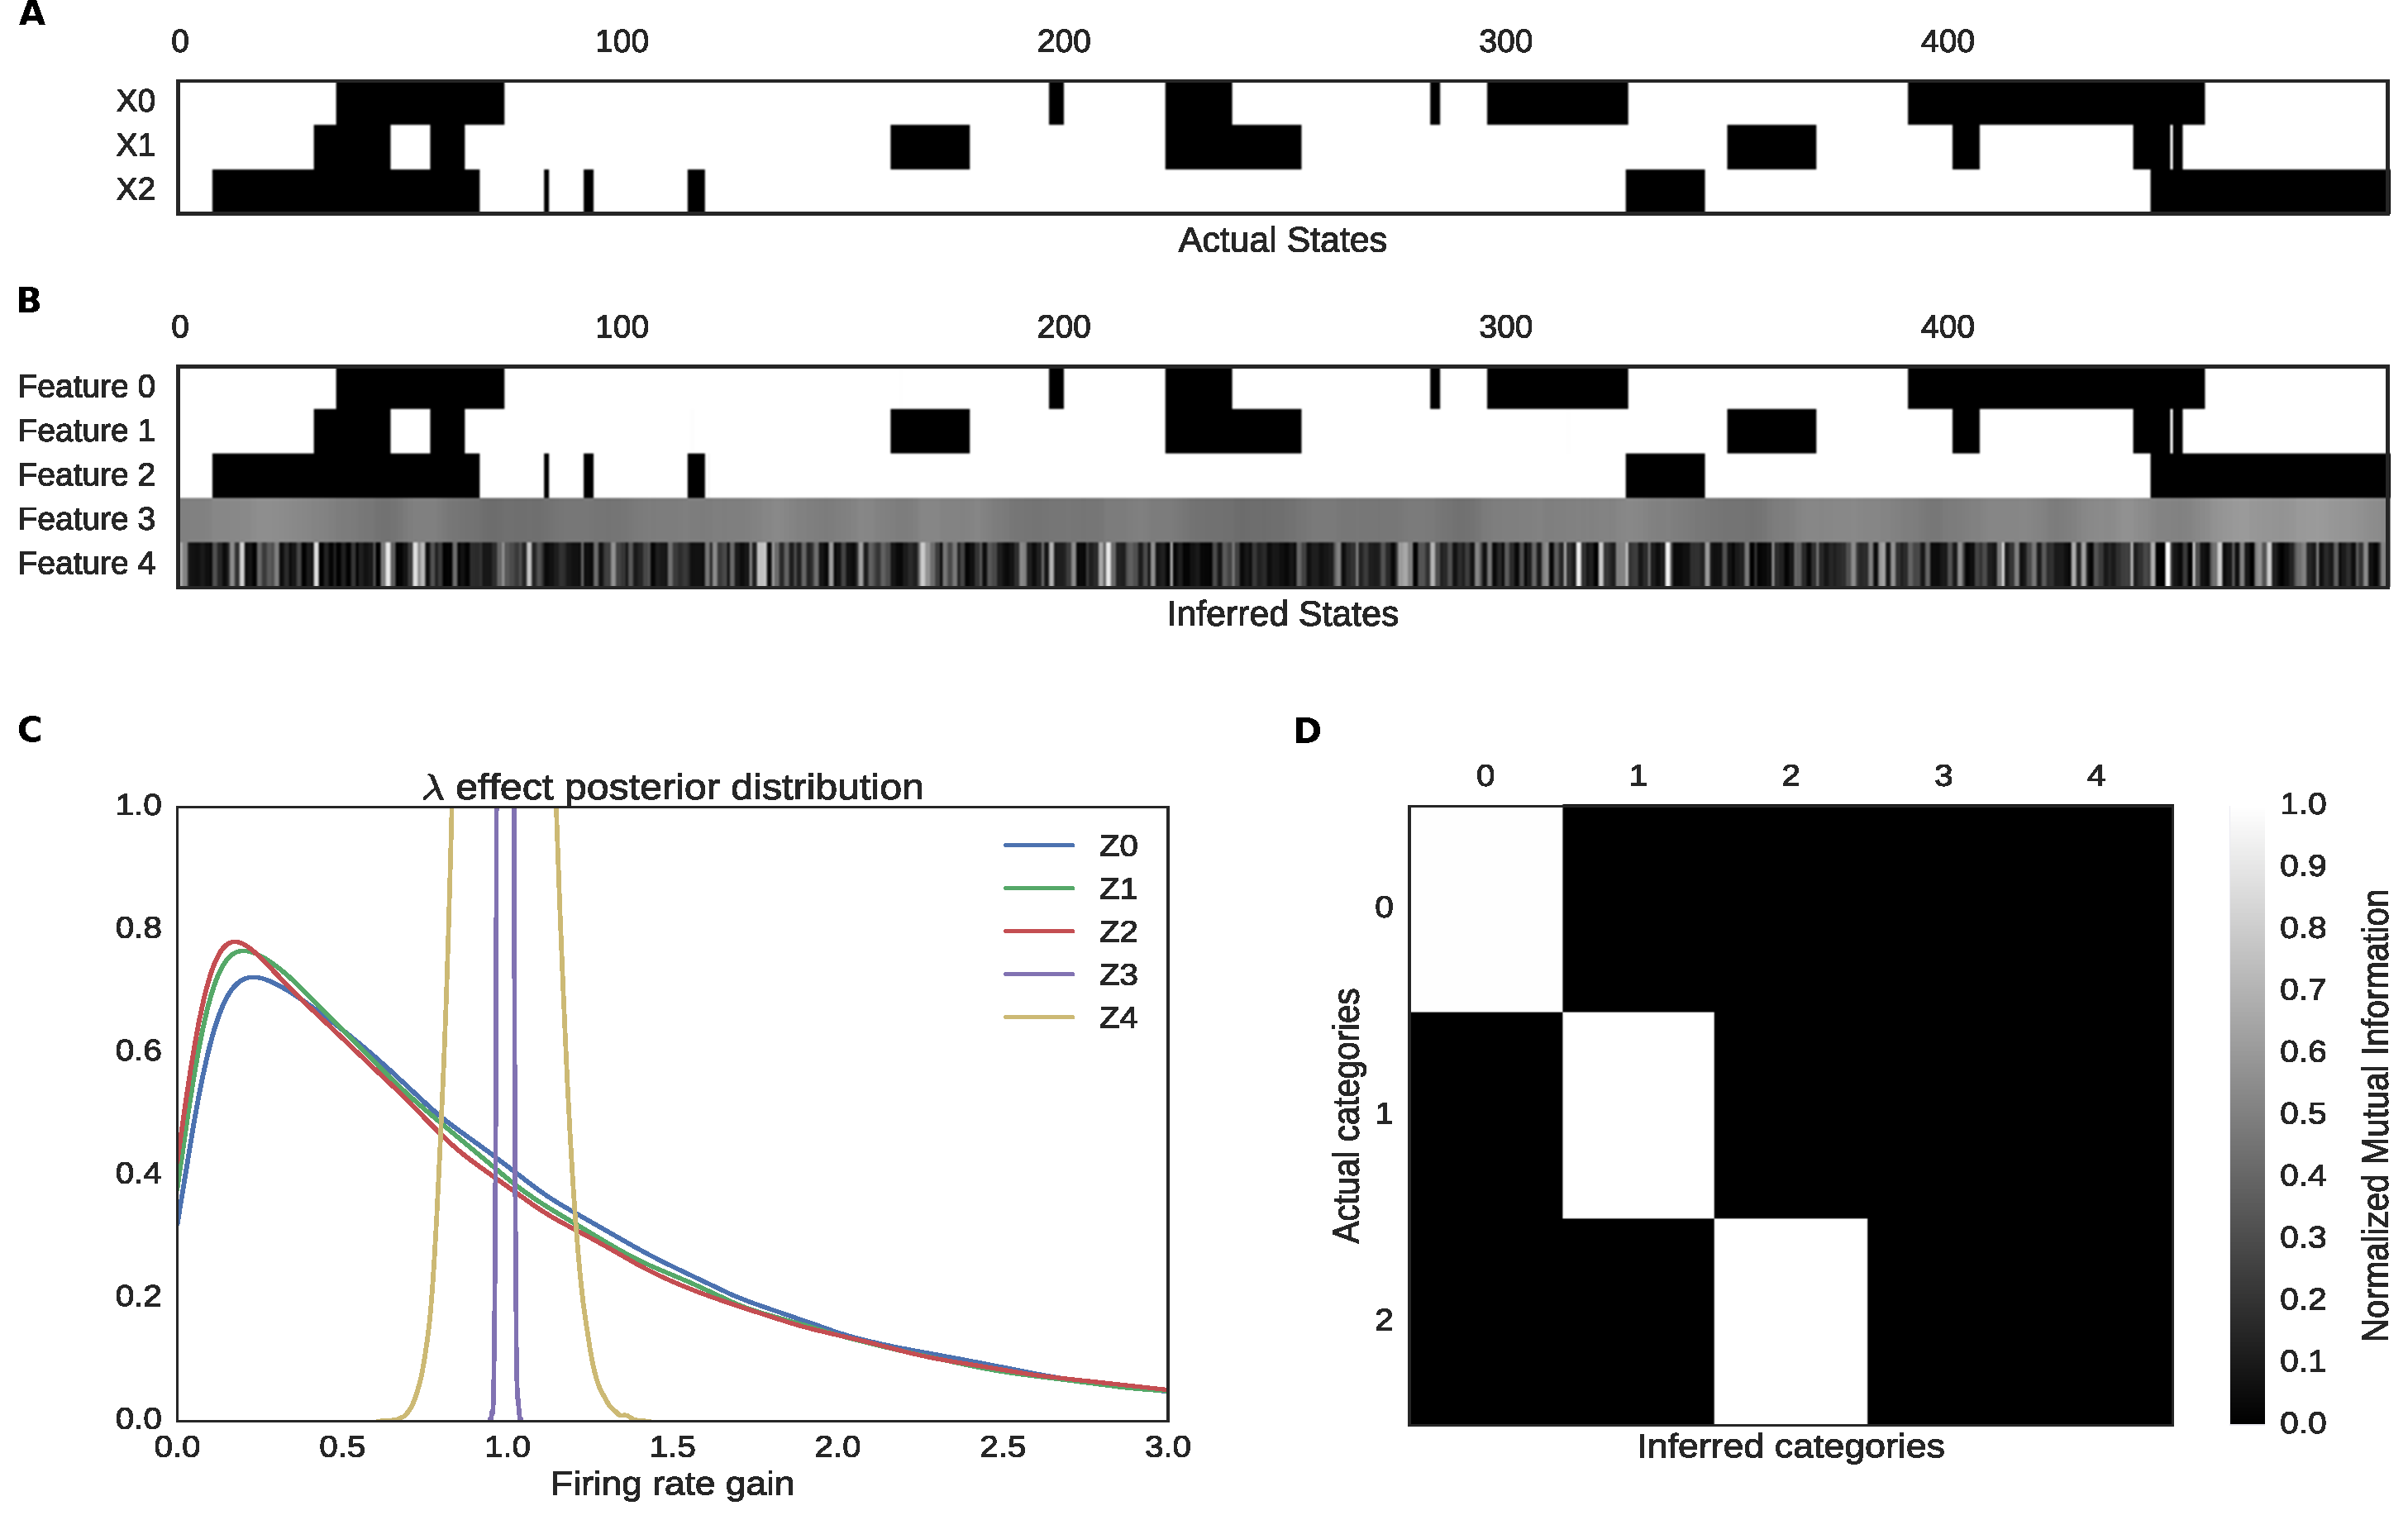
\includegraphics[width=1\linewidth]{synthetic}
    \caption{\textbf{Top:} Actual and recovered binary features for a subset of stimulus times in the dataset. Note that inferred feature 3 is the inverse of actual feature 0, and that unused features are in gray, indicating a high posterior uncertainty in the model. \textbf{Bottom left:} Population posterior distributions for $\lambda_z$. Features 0 and 1 are effectively point masses around gain 1 (no effect), while features 2--4 approximate the $\text{Ga}(1, 1)$ data-generating model. \textbf{Bottom right:} Normalized mutual information between actual and inferred states.}
    \label{synthetic}
\end{figure}

As seen in Figure \ref{synthetic}, the model correctly recovers only the features present in the original data. We quantified this by calculating the normalized mutual information $\hat{I}\equiv I(X, Y)/\sqrt{H(X)H(Y)}$, between the actual states and the inferred states, with $H(Z)$ and $I$ estimated by averaging the variational posteriors (both absolute and conditioned on actual states) across time. Note that superfluous features in the model have high posterior uncertainty for $z_k$ and high posterior confidence for $\lambda_{zk}$ around 1 (no effect). In addition, the model correctly recovers coefficients for the observed covariates, and when limited to fewer features than in the generating model, recovers a subset of the features accurately rather than blending features together (see Supplement).

\subsection{Labeled neural data}
We applied our model to a well-studied neural data set comprising single neuron recordings from macaque area LIP during the performance of a perceptual discrimination task \cite{roitman2002response}\footnote{Data available at \texttt{https://www.shadlenlab.columbia.edu/resources/RoitmanDataCode.html}}. In the experiment, stimuli consisting of randomly moving dots, some percentage of which moved coherently in either the preferred or anti-preferred direction of motion for each neuron. The animal's task was to report the direction of motion. Thus, in addition to 5 coherence levels, each trial also varied based on whether the motion direction corresponed to the target in or out of the response field as depicted in Fig. \ref{roitman}.\footnote{In the case of 0\% coherence, the direction of motion was inherently ambiguous and coded according to the monkey's eventual choice.}

We fit a model with $K = 10$ features and $U = 27$ units to neural responses from the 1-second stimulus presentation period of the task. Spike counts corresponded to bins of $dt = 20$ms. In this case, each unit experienced a different number of presentations of each stimulus condition, resulting in a ragged observation matrix. Figure \ref{roitman} shows the experimental labels from the concatenated stimulus periods, along with labels inferred by our model. Once again, the model has left some features unused, but correctly discerned differences between stimuli in the unlabeled data. Even more importantly, though given ten distinct stimulus classes, the model has clearly inferred the factorial design of the experiment, with the two most prominent features, $z_0$ and $z_1$, capturing the two levels of the crossed factor with the largest effect size: whether or not the relevant target is inside or outside the receptive field of the neuron. Moreover, the model correctly discriminates between two identical stimulus conditions (0\% coherence) based on the monkey's eventual decision (In vs Out). In addition, the model correctly captures the initial 200ms ``dead time'' during the stimulus period, in which firing rates remain at pre-stimulus baseline. Finally, the model uses the same features to describe stimuli with similar firing rates, as well as roughly capturing the time course of stimulus differentiation. As a result, mismatch between the ground truth labels and model-inferred features reflects fundamental ambiguities in the neural data, with the model's latent states taking into account features of spiking response not necessarily known in advance by experimenters.

\begin{figure}[ht]
    \center
    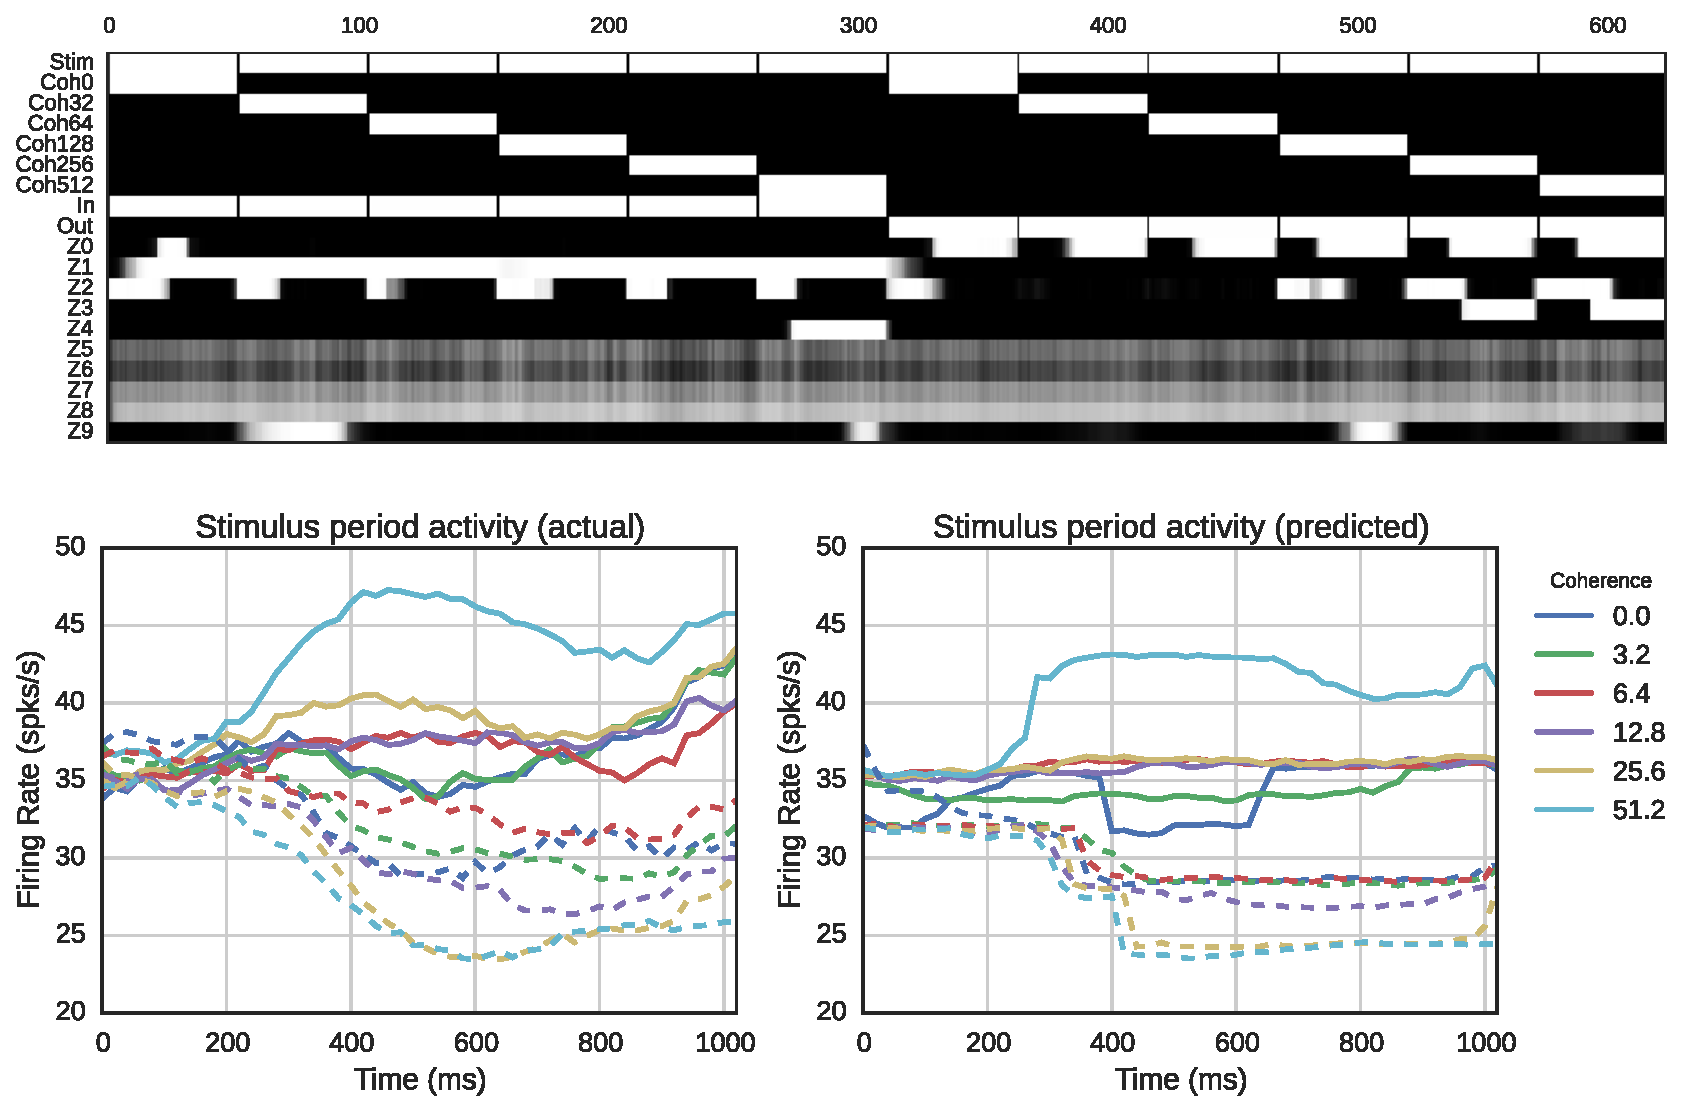
\includegraphics[width=1\linewidth]{roitman}
    \caption{\textbf{Top:} Actual and recovered binary features during the stimulus presentation period. Note that model features 5 -- 8 are unused and that feature 0 closely tracks the Out feature of the data, albeit delayed. \textbf{Bottom:} Actual and predicted firing rates for the stimulus period. Note that the model infers stimulus categories from the data, including appropriate timing of differentiation between categories.}
    \label{roitman}
\end{figure}

\subsection{Movie data}
Finally, we applied our model to a data set comprising single neuron recordings made in macaque monkeys as they freely viewed movies of primate social interactions in the wild%\cite{adams_inprep}
 . These video clips, collected from a rhesus macaque research field site, effectively represent the range of behaviorally relevant stimuli for macaques, including the four ``F''s of animal behavior: fighting, fleeing, foraging, and reproduction. Thus this dataset represents a rare opportunity for exploratory feature selection based on neural responses.

On each trial of the experiment, monkeys viewed a random 5-second clip from a movie database ($T \approx 5$h, $dt = 30$ frames/s). On the following trial, monkeys were given a two-alternative choices with options chosen from the set \{repeat clip, continue clip, blank screen, new clip\}. Since each neuron saw only a subset of clips within the database, and these clips began at with random offsets, observations were sparse, with total number of observations $N_{obs} = 7.42 \times 10^6$ and $\overline{M} = N_{obs}/T \approx 14$. These data form a particularly intriguing application of our model, since the neurons recorded were located in the orbitofrontal and dorsolateral prefrontal cortices, areas not normally associated with low-level visual processing. In fact, there is reason to believe that the relevant features encoded in these areas for such naturalistic stimuli are behavioral and social \cite{watson2012social}.

Because the behaviors of interest in these stimuli potentially span a large range of time scales, we used semi-Markov dynamics with a maximum duration of $D = 500$ on the latent states\footnote{We also allowed for self-transitions, potentially capturing behavior on even longer timescales.}. We fit a model with $K=10$ features and the same hierarchical priors on baselines and latent firing rate effects as in previous experiments. In addition, because many neurons in the data set exhibited a transitory increase in firing with movie onset on each trial (independent of movie content), we include this movie onset response as an external covariate $x(t)$ specific to each neuron. We calculated this separately for each recorded unit by averaging spike counts (relative to stimulus onset) across trials, smoothing, and taking the log so that $x(t)$ was coded as a multiplicative rather than an additive effect on firing. This can be loosely viewed as a means of preprocessing our data, in which we account for a large known effect by specifying it as a covariate in the model.

\begin{figure}[ht]
    \center
    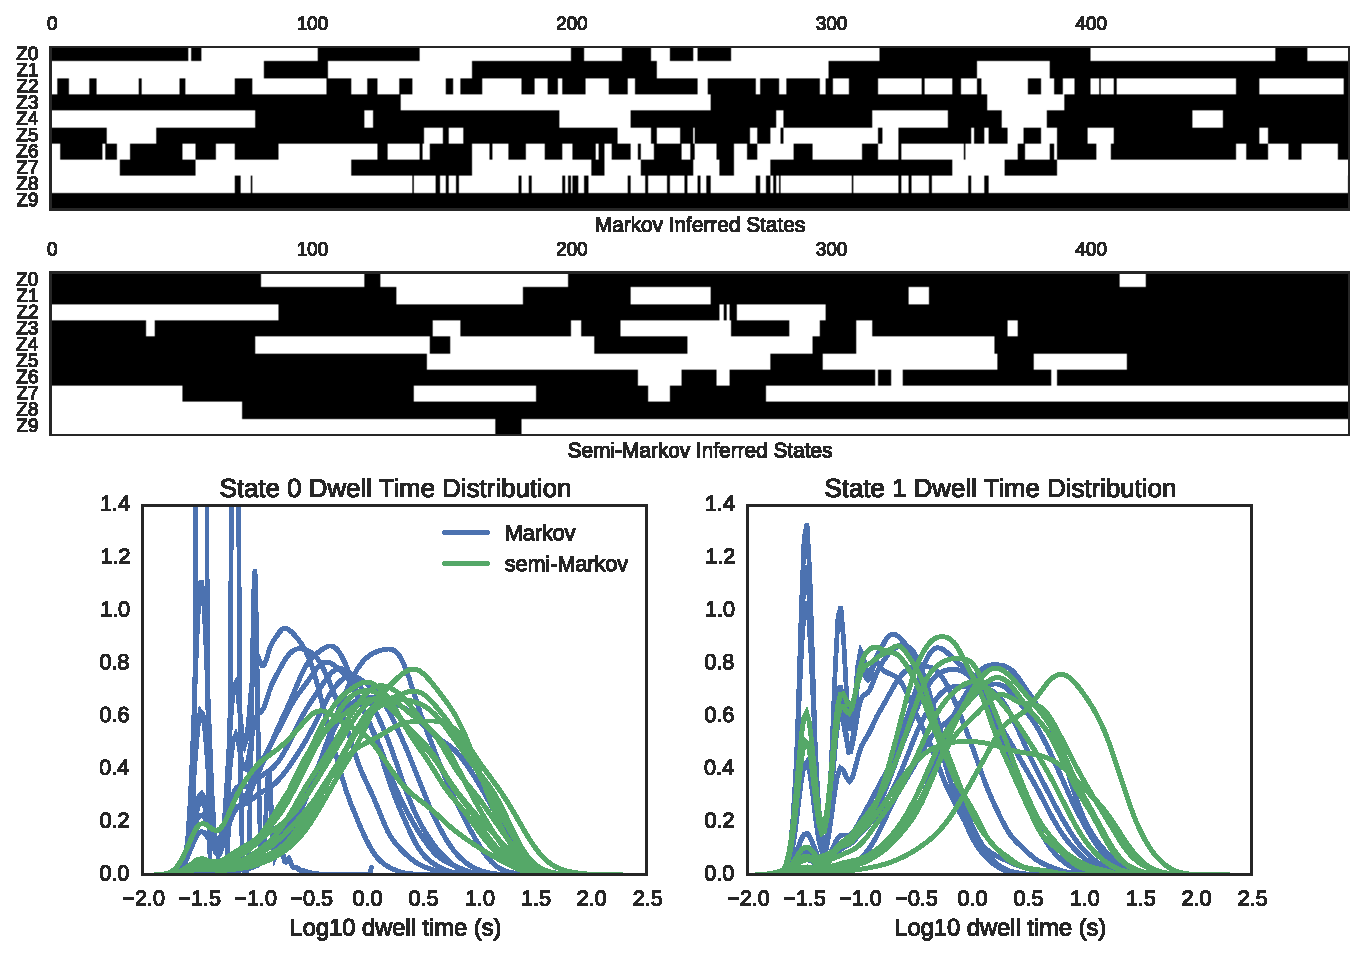
\includegraphics[width=1\linewidth]{movie_data}
    \caption{\textbf{Top:} Maximum \emph{a posterior} inferred features for the Markov and semi-Markov models. Plotted data are for the same stimulus for $\approx 17$s of data. \textbf{Bottom:} Estimated dwell time distributions for off (0) and on (1) states in the Markov and semi-Markov models. Dwell times include self-transitions. Dwell times for the Markov case (blue) are clearly lower than those for the semi-Markov case (green).}
    \label{movie_results}
\end{figure}

Figure \ref{movie_results} shows a comparison of Markov and semi-Markov models applied to feature detection in the stimulus set. Labels were calculated as maxima of posterior marginals, independently for each time bin. Clearly, the semi-Markov model captures the rich heterogeneity in the durations of stimulus-driven features in neural spiking, particularly in the on (1) state. This is also visible in the kernel density estimates, which show event durations on the order of tens of seconds for the semi-Markov model, as opposed to mere seconds in the Markov case. Thus semi-Markov models (and other models that take into account multiple timescales) will likely be necessary to capture variations in neural activity on the timescales relevant to natural behaviors.

\section{Discussion}
Here, we have proposed and implemented a method for learning features in stimuli via the responses of populations of spiking neurons. This work addresses a growing trend in systems neuroscience --- the increasing use of rich and unstructured stimulus sets --- without requiring either expert labeling or a metric on the stimulus space. As such, we expect it to be of particular use in disciplines like social neuroscience, olfaction, and other areas in which the real world is complex and strong hypotheses about the forms of the neural code are lacking. By learning features of interest to neural populations directly from neural data, we stand to generate unexpected, more potentially more accurate (less biased) hypotheses regarding the neural representation of the external world.  

We have shown that our model is capable of parsimoniously and correctly inferring features in the low signal-to-noise regime of cortical activity, even in the case of independently recorded neurons. Moreover, by employing a fully variational, Bayesian approach to inference, we gain three key advantages: First, we gain the advantages of Bayesianism in general: estimates of confidence in inferences, parsimony and regularization via priors, and the ability to do principled model comparison. Second, variational methods scale well to large datasets. Finally, variational methods are fast, in that they typically converge within only a few tens of iterations and in many case (such as ours) require mostly simple coordinate updates. 

Future directions include augmenting the model of overdispersion via an autoregressive process to take into account slow variations in neural activity not driven by the stimulus; adding non-trivial temporal dependence to latent variables in a manner consistent with kernels typically used with Poisson regression models; and an implementation of the model using stochastic variational inference for application to larger, next-generation neural data sets.

\subsubsection*{Acknowledgments}
This work was supported by an NIH Big Data to Knowledge Career Development Award to JP (K01ES025442). We wish to thank Geoff Adams and Michael Platt for generous use of their data.


\subsubsection*{References}
\begingroup
\footnotesize
\renewcommand{\section}[2]{}
\bibliography{pearson_beck}{}
\bibliographystyle{ieeetr}
\endgroup

\pagebreak

\setcounter{equation}{0}
\setcounter{figure}{0}
\setcounter{table}{0}
\setcounter{page}{1}
\setcounter{section}{0}
\makeatletter
\renewcommand{\theequation}{S\arabic{equation}}
\renewcommand{\thefigure}{S\arabic{figure}}

\part*{Supplementary Information}

\section{Evidence Lower Bound (ELBO)}
Here we derive the evidence lower bound (ELBO) used as a variational objective by our inference algorithm. That is, we want to calculate
\begin{equation}
    \mathcal{L} \equiv \mathbb{E}_q \left[\log \frac{p(\Theta|N)}{q(\Theta)} \right] = \mathbb{E}_q \left[\log p(\Theta|N) \right] + \mathcal{H}[q(\Theta)]
\end{equation}
From \cite{beal2003variational}, this can be written
\begin{multline}
    \mathcal{L} = \mathbb{E}_{q(\pi)} \left[\log \frac{p(\pi)}{q(\pi)} \right]
    + \mathbb{E}_{q(A)} \left[\log \frac{p(A)}{q(A)} \right]
    + \mathbb{E}_{q}\left[ \log \frac{p(N, z|\lambda, A, \pi)}{q(z)}\right] \\
    + \mathbb{E}_{q(\theta)} \left[\log \frac{p(\theta)}{q(\theta)} \right]
    + \mathbb{E}_{q(\lambda)} \left[\log \frac{p(\lambda)}{q(\lambda)} \right]
    + \mathbb{E}_{q(\gamma)} \left[\log \frac{p(\gamma)}{q(\gamma)} \right]
\end{multline}
For the first two terms, updates are standard and covered in \cite{beal2003variational}. The rest we do piece-by-piece below:

\subsection{Log evidence}
We would like to calculate $\mathbb{E}_{q}\left[ \log \frac{p(N, z|x, \Theta)}{q(z)}\right]$. To do this, we make use of expectations calculated via the posteriors returned from the forward-backward algorithm
\begin{align}
    \xi_{t} &\equiv p(z_{t}|N, \theta) &
    \Xi_{t, ij} &\equiv p(z_{t+1} = j, z_{t} = i|N, \theta) &
    \log Z_{t} &= \log p(N_{t+1}|N_{t}, \Theta)
\end{align}
Here, we have suppressed the latent feature index $k$ and abuse notation by writing the observation index as $t$, but in the case of multiple observations at a given time, we pool across units and presentations: $N_t \equiv \sum_{m; t(m) = t} N_m$. From this, we can write
\begin{multline}
     \mathbb{E}_{q}\left[ \log p(N, z|x, \Theta) \right] =
     \sum_{mkr} \left[N_m \left(
        \overline{\log \theta_m} + \overline{\log \lambda_{0u(m)}} +
        \xi_{t(m)k}\overline{\log \lambda_{zuk}} +
        x_{t(m)r} \overline{\log \lambda_{xu(m)r}}
     \right) \right] \\
     - \sum_m \overline{\theta_m} \mathbb{E}_q\left[\Lambda_{t(m)u(m)} \right]      + \sum_{tk} \left[ \text{tr}\left(\Xi_{tk} \overline{\log A_k^T} \right)
     + \xi_{0k}^T \overline{\log \pi_k}
     \right]
    + \text{constant}
 \end{multline}
In what follows, we will drop the irrelevant constant. For $\overline{\log y}$, where $y \in \lbrace \theta, \lambda_0, \lambda_z, \lambda_x \rbrace$, the assumption $q(y) = \text{Ga}(\alpha, \beta)$ gives
\begin{equation}
    \overline{\log y} = \psi(\alpha) - \log \beta
\end{equation}
with $\psi(x)$ the digamma function. Likewise, the expectation $\overline{\theta}$ is straightforward. For the expectation of the rate, we have
\begin{equation}
    \label{eff_rate}
    \mathbb{E}_q\left[
        \lambda_{0u} \prod_k \lambda_{zuk}^{z_{tk}} \prod_r \lambda_{xur}^{x_{tr}}
    \right] = \frac{\alpha_{0u}}{\beta_{0u}}
    \prod_k \left(1 - \xi_{tk} + \xi_{tk} \frac{\alpha_{zuk}}{\beta_{zuk}} \right)
    \prod_r \frac{1}{\beta_{xur}^{x_{tr}}} \frac{\Gamma(\alpha_{xur} + x_{tr})}{\Gamma(\alpha_{xur})}
\end{equation}
However, for $\alpha \gg x$, we have $\Gamma(\alpha + x)/\Gamma(\alpha) \approx \alpha^x$, so that we can write
\begin{equation}
    \label{HFG}
    \mathbb{E}_q[\Lambda_{tu}] = H_{0u} F_{tu} G_{tu}
\end{equation}
with $G_{tu} \approx \prod_r (\alpha_{xur}/\beta_{xur})^{x_{tr}}$. In addition, it will later be useful to have the expectation over \emph{all except} a particular feature $k$ or $r$, for which we define
\begin{align}
    \label{F}
    F_{tuk} &\equiv \prod_{k'\neq k} \left(1 - \xi_{tk'} + \xi_{tk'} \frac{\alpha_{zuk'}}{\beta_{zuk'}} \right) \\
    \label{G}
    G_{tur} &\equiv \prod_{r' \neq r} \left(\frac{\alpha_{xur'}}{\beta_{xur'}} \right)^{x_{tr'}}
\end{align}
Finally, we want the entropy of the variational posterior over $z$, $\mathbb{E}_q[-\log q(z)]$. We can write this in the form
\begin{equation}
    -\sum_{tk} \left[
        \xi_{tk}^T\eta_{tk} + \text{tr}\left(\Xi_{tk} \tilde{A}_k^T \right)
        + \xi_{0k}^T\tilde{\pi}_k
        - \log Z_{tk}
    \right]
\end{equation}
with $(\eta, \tilde{A}, \tilde{\pi})$ the parameters of the variational posterior corresponding to the emission, transition, and initial state probabilities of the Markov chain (interpreted as matrices) and $Z$ the normalization constant. From \cite{beal2003variational}, we have that variational updates should give
\begin{align}
    \tilde{A}_k &\leftarrow \overline{\log A_k} &
    \tilde{\pi}_k &\leftarrow \overline{\log \pi_k}
\end{align}
while the effective emission probabilities are
\begin{align}
    \eta_{tk} &\leftarrow \delta_{z_{tk}, 1}\cdot \sum_{m; t(m) = t} N_m \overline{\log \lambda_{zu(m)k}} - \sum_{m; t(m) = t} \overline{\theta_m} H_{0u(m)} F_{tku(m)} G_{tu(m)}
\end{align}
Given these update rules, we can then alternate between calculating $(\eta, \tilde{A}, \tilde{\pi})$, performing forward-backward to get $(\xi, \Xi, \log Z)$ and recalculating $(\eta, \tilde{A}, \tilde{\pi})$.

\subsection{Overdispersion, firing rate effects}
Both the case of $p(\theta)$ and $p(\lambda)$ are straightforward. If we ignore subscripts and write $p(y) = \text{Ga}(a, b)$, $q(y) = \text{Ga}(\alpha, \beta)$, then
\begin{equation}
    \mathbb{E}_q \left[\log \frac{p(y)}{q(y)} \right] =
    (\overline{a} - 1) \overline{\log y} + \overline{b} \overline{y} + \mathcal{H}[q(y)]
\end{equation}
where again, $\overline{\log y}$, $\overline{y}$ and $\mathcal{H}[q(y)]$ are straightforward properties of the gamma distribution. Expectations of the prior parameters are listed in Table \ref{expectation_table}. Note in the last line that there is no expectation, since we have not assumed a hierarchy over firing rate effects for the covariates, $x$.
\begin{table}[ht]
\caption{Expectations of prior parameters for overdispersion and firing rates}
\label{expectation_table}
\begin{center}
\begin{tabular}{lcc}
\multicolumn{1}{c}{\bf Variable}  &\multicolumn{1}{c}{\bf $\mathbb{E}_q[a]$} &\multicolumn{1}{c}{\bf $\mathbb{E}_q[b]$}
\\ \hline
$\theta$ &$\overline{s}$ &$\overline{s}$ \\
$\lambda_0$ &$\overline{c_0}$ &$\overline{c_0 d_0}$ \\
$\lambda_z$ &$\overline{c_z}$ &$\overline{c_z d_z}$ \\
$\lambda_x$ &$a_x$ &$b_x$ \\
\end{tabular}
\end{center}
\end{table}
As we will see below, the expectations under the variational posterior of $s$, $c$, and $d$ are themselves straightforward to calculate.

\subsection{Hyperparameters}
As shown in the main text, the hyperparameters $c$ and $d$, given gamma priors, have conjugate gamma posteriors, so that their contribution to the evidence lower bound, $\mathbb{E}_q \left[\log \frac{p(\gamma)}{q(\gamma)} \right]$ is a sum of terms of the form
\begin{align}
    (a_{c} - 1) \overline{\log c} + b_{c} \overline{c} + \mathcal{H}[q(c)] +
    (a_{d} - 1) \overline{\log d} + b_{d} \overline{d} + \mathcal{H}[q(d)]
\end{align}
In other words, these are straightforward gamma expectations, functions of the prior parameters $a$ and $b$ for each variable and the corresponding posterior parameters $\alpha$ and $\beta$. Similarly, the overdispersion terms are exactly the same with the substitutions $a \rightarrow s$, $d\rightarrow 1$.

\section{Inference}
\subsection{Conjugate updates}
For updates on the overdispersion, firing rate, and hyperparameter variables, we have the simple conjugate update rules depicted in Table \ref{conj_updates}. These can be derived either from free-form variational arguments, or exponential family rules, but are in any case straightforward\cite{Blei2006-oh}. If we assume a $\text{Ga}(a, b)$ prior and $\text{Ga}(\alpha, \beta)$ variational posterior, all of these have a simple algebraic update in terms of sufficient statistics.

\begin{table}[ht]
\caption{Conjugate updates for Gamma distributions}
\label{conj_updates}
\begin{center}
\begin{tabular}{lcc}
\multicolumn{1}{c}{\bf Variable}  &\multicolumn{1}{c}{\bf $\alpha - a$} &\multicolumn{1}{c}{\bf $\beta - b$}
\\ \hline
$\theta_m$         &$N_m$  &$H_{0u(m)}F_{t(m)u(m)}G_{t(m)u(m)}$ \\
$s_u$         &$\frac{1}{2}\sum_m \delta_{u(m), u}$  &$\sum_m \delta_{u(m), u} [\overline{\theta_m} - \overline{\log \theta_m} - 1]$ \\
$\lambda_{0u}$         &$\sum_{t} N_{tu}$  &$\overline{\theta}_u H_{0u}\sum_t F_{tu}G_{tu}$ \\
$\lambda_{zuk}$         &$\sum_t N_{tu} \xi_{tk}$  &$\overline{\theta}_u H_{0u}\sum_t F_{tuk}G_{tu}$ \\
$\lambda_{xur}$         &$\sum_t N_{tu} x_{tr}$  &cf. Section \ref{non-conj} \\
$c_{0}$         &$U/2$  &$\sum_u\mathbb{E}_q \left[d_{0} \lambda_{0u} - \log \lambda_{0u} - \log d_{0} - 1\right]$ \\
$c_{zk}$         &$U/2$  &$\sum_u\mathbb{E}_q \left[d_{zk} \lambda_{zuk} - \log \lambda_{zuk} - \log d_{zk} - 1\right]$ \\
$c_{xr}$         &$U/2$  &$\sum_u\mathbb{E}_q \left[d_{xr} \lambda_{xur} - \log \lambda_{xur} - \log d_{xr} - 1\right]$ \\
$d_{0}$         &$U\mathbb{E}_q[c_{0}]$  &$\sum_u\mathbb{E}_q \left[c_{0}\lambda_{0u}\right]$ \\
$d_{zk}$         &$U\mathbb{E}_q[c_{zk}]$  &$\sum_u\mathbb{E}_q \left[c_{zk}\lambda_{zuk}\right]$ \\
$d_{xr}$         &$U\mathbb{E}_q[c_{xr}]$  &$\sum_u\mathbb{E}_q \left[c_{xr}\lambda_{xur}\right]$ \\
\end{tabular}
\end{center}
\end{table}

Here, we overload notation to write $N_{tu} = \sum_m \delta_{u(m), u} \delta_{t(m), t}\, N_m$, $\overline{\theta}_u = \sum_m \delta_{u(m), u}\overline{\theta}_m$, and make use of $H$, $G$, and $F$ as defined in \ref{HFG} - \ref{G}. Indeed, our implementation caches $F$ and $G$ for a substantial speedup (at the cost of additional memory requirements).

\subsection{Non-conjugate updates}
\label{non-conj}
We employ explicit optimization steps for two updates in our iterative Algorithm \ref{algo}. In each case, we employ an off-the-shelf optimization routine, though more efficient alternatives are likely possible.

\subsubsection{Covariate firing rate effects}
\label{beta_x}
Because we do not restrict the covariates $x(t)$ to be binary, the expression \ref{eff_rate}, no longer yields a conditional log probability for $\lambda_x$ in the exponential family. This leaves us with a transcendental equation to solve for $\beta_{xr}$. However, from Table \ref{conj_updates}, we see that $\alpha_{xr} \gg \sum_t x_{tr}$, allowing us to approximate $G_t \approx \prod_r (\alpha_{xr}/\beta_{xr})^{x_{tr}}$ as we have done above. Moreover, since the sum $\sum_t G_t \sim T\overline{G}$, we expect $\alpha_x / \beta_x \approx 1$ at the optimum for most reasonable datasets. We thus reparameterize $\beta_{xur} = \alpha_{xur}e^{-\epsilon_{ur}}$ and write the relevant $\epsilon$-dependent piece of the objective function $\mathcal{L}$ as
\begin{equation}
    \mathcal{L}_\epsilon = \sum_{ur} \left[a_{xur}\epsilon_{ur} - b_{xur}e^{-\epsilon_{ur}} \right] - \sum_m \overline{\theta}_m H_{0u(m)} F_{t(m)u(m)}
    e^{-\sum_r \epsilon_{u(m)r} x_{t(m)u(m)r}}
\end{equation}
We also supply the optimizer with the gradient:
\begin{equation}
    \nabla_\epsilon \mathcal{L}_\epsilon = a_{xur} - b_{xur}e^{-\epsilon_{ur}}  - \sum_{m; u(m) = u} x_{t(m)ur} \overline{\theta}_m H_{0u} F_{t(m)u}
    e^{-\sum_r \epsilon_{ur} x_{t(m)ur}}
\end{equation}
where we sum only over observations with $u(m) = u$. On each iterate, we then optimze $\mathcal{L}_\epsilon$, initialzing $\beta_x$ to the just-updated value of $\alpha_x$. In addition, we do not update firing rate effects for covariates separately, but optimize $\beta_{xur}$ for all $r$ together. Again, more efficient schemes are no doubt possible.

\subsubsection{Semi-Markov duration distribution}
If the dwell time distributions of states in the semi-Markov model were truly continuous, the parameters $(m, s^2)$ of a lognormal distribution $p(d|j)$ would have a Normal-Gamma conjugate prior, and updates would be closed-form. However, the requirement that the durations be integers and that there exist a maximal duration, $D$, over which these probability mass functions must normalize results in an extra term in $\mathbb{E}_q[\log p]$ arising from the normalization constant. In this case, we must explicitly optimize for the parameters of the Normal-Gamma prior on $(m, s^2)$. However, unlike the case of \ref{beta_x}, these parameters are only updated for one latent feature at a time. Since the Normal-Gamma distribution has only 4 parameters and the number of states of the latent variable is $S = 2$, this requires updating $4SK$ parameters, but only taken $4S = 8$ at a time, a much more manageable task.

To derive the optimization objective, we begin by noting that, to terms proportional to $\Xi$ and $\xi_0$ in the expectation of the latent state dynamics, the semi-Markov model adds an additional term
\begin{multline}
    \sum_{d j k} C(d, j, k) \mathbb{E}_q \left[\log p_k(d|j) - \log \left(\sum_{d=1}^D p_k(d|j) \right) \right] \ge \\
    \sum_{d j k} C(d, j, k) \left[\mathbb{E}_q \left[\log p_k(d|j)\right] - \log \sum_{d=1}^D \mathbb{E}_q\left[p_k(d|j) \right] \right]
\end{multline}
where $d$ is the duration variable, $j$ labels states of the chain (here 0 and 1), and $k$, as elsewhere, labels chains\cite{Mitchell1993-sl,Mitchell1995-go,Yu2006-bb}. $C$ is defined for each state and chain as the probability of a dwell time $d$ in state $j$ \emph{conditioned on} the event of just having transitioned to $j$\footnote{Thus $C$ is equivalent to $\mathcal{D}_{t|T}$ in \cite{Yu2006-bb}.}
\footnote{
We also note that, just as the emission, transition, and initial state probabilities have their counterparts in variational parameters $(\eta, \tilde{A}, \tilde{\pi})$ in $q(z)$, so $C$ is matched by a term $-\sum_{djk} C(d, j, k) \nu_{djk}$ in $\mathbb{E}_q[-\log q]$. And in analogy with the HMM case, variation with respect to $\nu$ gives
\begin{equation}
    \nu_{djk} = \mathbb{E}_q \left[\log p_k(d|j)\right] - \log \sum_{d=1}^D \mathbb{E}_q\left[p_k(d|j) \right],
\end{equation}
implying that there are cancellations between $\log p(N, z|\Theta)$ and $\log q(z)$ in $\mathcal{L}$ and care must be taken when calculating it\cite{beal2003variational}.}

Thus the objective to be optimized is
\begin{equation}
    \sum_{d j k} C(d, j, k) \left[\mathbb{E}_q \left[\log p_k(d|j)\right] - \log \sum_{d=1}^D \mathbb{E}_q\left[p_k(d|j) \right] \right] + \mathbb{E}_q\left[\log \frac{p(m, \tau)}{q(m, \tau)} \right]
\end{equation}

For the case of $p(d|m, s^2)$ lognormal and $(m, \tau = s^{-2})$ Normal-Gamma, the terms $\mathbb{E}_q[\log p(d)]$ involve only routine expectations of natural parameters of the Normal-Gamma, and similarly for the expected log prior and entropy in the last term. Only slightly more complicated is the term arising from the normalization constant, which in the standard $(\mu, \lambda, \alpha, \beta)$ parameterization of the Normal-Gamma takes the form
\begin{equation}
    \mathbb{E}_q[p(d|m, \tau)] = \int d\tau dm \; p(d|i, m, \tau) q(m, \tau)
    = \frac{1}{\sqrt{2\pi}d} \sqrt{\frac{\lambda}{1 + \lambda}}
    \frac{\Gamma(\alpha + 1/2)}{\Gamma(\alpha)}
    \frac{\beta^{-\frac{1}{2}}}{\hat{\beta}^{\alpha + \frac{1}{2}}}
\end{equation}
with
\begin{equation}
    \hat{\beta} \equiv 1 + \frac{1}{2\beta} \frac{\lambda}{1 + \lambda}
    (\log d - \mu)^2
\end{equation}
This can be derived either by performing the integral directly or by noting that the result should be proportional to the posterior (Normal-Gamma, by conjugacy) of $(m, \tau)$ after having observed a single data point, $\log d$.

\begin{algorithm}[ht]
\caption{Iterative update for variational inference}\label{algo}
\begin{algorithmic}[1]
\Procedure{Iterate}{}
    \State Update baselines $\lambda_0$\Comment{conjugate Gamma}
    \State Update baseline hyperparameters $\gamma_0$\Comment{conjugate Gamma}
    \For{$k = 1\ldots K$}
        \State Update firing rate effects $\lambda_{zk}$\Comment{conjugate Gamma}
        \State Update firing rate hyperparameters $\gamma_{zk}$\Comment{conjugate Gamma}
        \State Calculate expected log evidence $\eta_k$
        \State Update Markov chain parameters $\tilde{A}_k, \tilde{\pi}_k$
        \State $\xi_k, \Xi_k, \log Z_k \gets$\Call{forward-backward}{$\eta_k, \tilde{A}_k, \tilde{\pi}_k$}
        \If{semi-Markov}
            \State Update duration distribution $p_k(d|j)$\Comment{BFGS optimization}
        \EndIf
        \State Update cached $F$
    \EndFor
    \State Update covariate firing effects $\lambda_x$\Comment{BFGS optimization}
    \State Update cached $G$
    \State Update overdispersion $\theta$\Comment{conjugate Gamma}
\EndProcedure
\end{algorithmic}
\end{algorithm}



\end{document}
